\documentclass[border=0pt]{standalone}
% \usepackage{pgfplots}
% \pgfplotsset{width=\linewidth,compat=3.1.10}
% \usepackage{pgfplotstable}
% \pgfplotsset{width=\linewidth,compat=1.8}
\usepackage{amsfonts}
\usepackage{amsmath}
\usepackage{tikz}
% \usetikzlibrary{shapes.geometric}
\usetikzlibrary{decorations.pathreplacing} % Load the decorations library
% \usetikzlibrary{arrows.meta}
\begin{document}
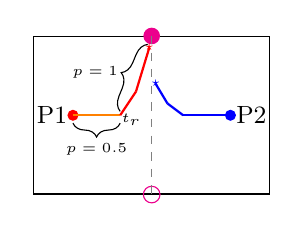
\begin{tikzpicture}
    \draw (0,0)  node[minimum height=2cm,minimum width=3cm,draw] (A) {};
    \fill[blue]  (1, 0) circle(2pt);
    \node[right] at (0.95, 0) {\small P2};
    \fill[red]  (-1, 0) circle(2pt);
    \node[left] at (-0.95, 0) {\small P1};
    \fill[magenta] (A.north) circle(3pt);
    \draw[magenta] (A.south) circle(3pt);
    % \node[below left] at (-1.4, -0.9) (l) {\tiny -1};
    % \node[below right] at (1.4, -0.9) (l) {\tiny 1};
    % \node[above left] at (-1.4, 0.9) (l) {\tiny -1};
    % \node[above right] at (1.4, 0.9) (l) {\tiny 1};
    \draw[orange, thick] (-1, 0) -- (-0.4, 0);
    % \node[below] at(-0.7, -0.2) {\tiny p=0.5};
    \node[below] at (-0.26, 0.14) {\tiny $t_r$};
    \draw[red, thick] (-0.4, 0) -- (-0.2, 0.3);
    \draw[red, thick] (-0.2, 0.3) -- (-0.03, 0.86) node {\tiny $\star$};
    \draw[blue, thick] (1, 0) -- (0.4, 0);
    \draw[blue, thick] (0.4, 0) -- (0.2, 0.15);
    \draw[blue, thick] (0.2, 0.15) -- (0.05, 0.4) node {\tiny $\star$};
    \draw[gray, dashed] (A.north) -- (A.south);
    
    % Add curly brace above the orange line
    \draw[
        decorate, 
        decoration={brace, amplitude=5pt, mirror}
    ] 
    (-1, -0.1) -- (-0.4, -0.1) node[midway, below=4pt] {\tiny $p=0.5$};

    \draw[
        decorate, 
        decoration={brace, amplitude=5pt}
    ] 
    (-0.4, 0.05) -- (-0.05, 0.9) node [midway, xshift=-14pt, yshift=2pt] {\tiny $p=1$};
\end{tikzpicture}
\end{document}
